% GENERATED FROM typst/manual/sections/03_temporal_observation.typ BY scripts/typ2tex.py (v1.0.0) — DO NOT EDIT.
% Edit canonical Typst under typst/ and regenerate with: python3 scripts/typ2tex.py --root . --outdir latex

\section{Temporal records and SI mapping}\label{manual:m3-temporal}

\paragraph{Setup: native input, observation domain, and five-boundary stack.}
To isolate native coupled recurrence from conditional SI unit stipulation and held-out
transfer falsification, declare the five-boundary metrology stack

\[
B_{\mathrm{pair}}(0,30]\to B_{\mathrm{lag}}\to B_{\mathrm{bridge}}\to B_{\mathrm{val}}\to B_{\mathrm{ext}}.
\]

Inside $B_{\mathrm{pair}}(0,30]\to B_{\mathrm{lag}}$, the temporal adapter
consumes the admitted recurrent waves and repeated coupled returns of
\mainequation{main:eq:wave-update-trace}, \mainequation{main:eq:coupling-trace}, and
\mainequation{main:eq:rcd-additive-realization}. Every bound record retains population,
preparation, directed couplings, complete committed prefixes, pending returns, integer
window endpoints, signed phase bias, lag, and directional reflection count; directional
RCD, bias, lag, and drift are recomputed directly from those committed records. Structural
RD belongs to each retained support, whereas duration participation requires a compatible
window map and is never supplied by a bare reclosure count. Displacement traversals,
hinges, dwells, emitted ticks, and returned clicks keep separate counts, and positive
reclosure counts without repeated cross-returns do not supply RCD. Two named readouts
replaying one context share its history rather than yielding independent samples, and
changing population, current, or window requires full replay rather than a cached scalar.

On the worked half-open window $(0,30]$, the compared lineage has four closures at cuts
$2,10,18,26$ and the reference lineage has three closures at cuts $2,12,22$.
Excluding the initial origin closure of each recurrent lineage yields reclosure increments
$(3,2)$, cadence ratio $\operatorname{biz}_{i|j}=3/2$ (reverse $2/3$),
additive directional durations $5$ and $7$ ($RD=3$ with directional reflection counts
$(1,1)$ versus $(2,2)$ in the declared native count domain), and biases
$(1/4,-1/4)$ giving unwrapped lag $3/2$ (reverse $-3/2$).

\paragraph{Derivation: declared apparatus bridge, conditional SI units, and gain non-identifiability.}
Crossing $B_{\mathrm{bridge}}$ under
\mainsection{main:subsec:m3-conditional-si-interface}, an explicit apparatus observation
map $\mathcal{O}_i$ (\mainequation{main:eq:m3-observation-map}) sends reference history
$\Gamma_R$, window $\omega$, population $\mathcal{P}$, coupling history $E$, and preparation to
corrected Cs-referenced cycle equivalents, anchoring conditional duration via
\mainequation{main:eq:m3-conditional-si-anchor} and
\mainequation{main:eq:m3-cs133-tau-interface}:

\begin{equation}\label{eq:manual-m3-cycle-bridge}
\hat{C}_{\mathrm{Cs}}=g_{\theta}(\Gamma_R,\omega,\mathcal{P},E,\mathrm{preparation}),\qquad\hat{T}=\frac{\hat{C}_{\mathrm{Cs}}}{\Delta\nu_{\mathrm{Cs}}}.
\end{equation}

The exact defining frequency converts cycle equivalents to seconds, while the first map
requires its own observation and calibration evidence and never assigns a universal
duration to a native cut. The general map $\mathcal{O}_i$ stays distinct from its affine
specialization $C_i^{\mathrm{aff}}=g_iq_i(\omega)+\delta_{\mathrm{end},i}$
($g_i>0$), and structural support scale, window extent, native cadence
(\mainequation{main:eq:wavelet-reference-timing}), observed turns, and SI frequency
remain separately typed. For stipulated cycle-equivalent gains $a_c,a_r>0$ per native
return and defining reference
$f_{\mathrm{Cs}}=9\,192\,631\,770\,\mathrm{Hz}$ (without a physical
clock realization), the fixed-window bridge evaluates

\[
T=\frac{a_rN_r}{f_{\mathrm{Cs}}},\qquad\bar{\nu}_c=\frac{a_cN_c}{T},\qquad t_1=t_0+T.
\]

The mapping binds both gains, coordinate and epoch, complete input records, defining
reference, and executable specification. At unit gain $a_c=a_r=1$, the worked pair
gives $T=2/f_{\mathrm{Cs}}=1/4596315885\,\mathrm{s}$ and
$\bar{\nu}_c=3f_{\mathrm{Cs}}/2=13788947655\,\mathrm{Hz}$. This
finite-window average and its derived reciprocal $1/\bar{\nu}_c$ supply no
independent validation; physical realization and drift, endpoint-phase, cycle-slip, and
temporal-dependence uncertainties stay unspecified, and gains are stipulated without
fitting hydrogen.

Because the countermodel family $g_{\lambda}(Z)=1+\lambda(55-Z)/54$
($\lambda>-1$) satisfies $g_{\lambda}(55)=1$ and $g_{\lambda}(1)=1+\lambda$, the
$\lambda=0$ and $\lambda=1$ models preserve both the native records and the Cs anchor
while emitting distinct reports; relative gain therefore stays unidentified. Known
hydrogen values remain retrospectively exposed. Evaluation validates each frozen
prediction against its bound model inputs before target comparison, binds separate
prediction and target hashes (changing only the target alters the diagnostic residual
without touching prediction bytes), and freezes the uncertain input model, readouts,
reduction, candidate selection, stopping rule, and comparison criterion in a separately
bound plan whose mutation invalidates replay; a later freeze cannot render earlier target
exposure blind, and an atomic point prediction with complete uncertainty remains
unresolved.

\paragraph{Specialization: held-out cross-field transfer, population controls, and causal intervention.}
At $B_{\mathrm{val}}$, the retained direct-coupling transfer experiment calibrates on
its first half and validates on its second; each half carries exactly
$N_{0,\mathrm{cal}}=N_{0,\mathrm{val}}=32$ reference reclosures. Freezing
$k_i=32/N_{i,\mathrm{cal}}$ predicts
$\hat{N}_{0,\mathrm{val}}=k_iN_{i,\mathrm{val}}$ on the held-out half
(\tabref{tab:manual-m3-anchor-transfer}).

\begin{table}[H]
\centering
\caption{Frozen gains and subsequent reference-count transfer ($N_{0,\mathrm{val}}=32$).}
\label{tab:manual-m3-anchor-transfer}
{\small
\begin{tabular}{lrrrr}
\toprule
Field & $N_{i,\mathrm{cal}}$ & $N_{i,\mathrm{val}}$ & $\hat{N}_{0,\mathrm{val}}$ & $(\hat{N}_{0,\mathrm{val}}-32)/32$ \\
\midrule
A & 58 & 48 & $768/29$ & $-5/29$ \\
B & 151 & 102 & $3264/151$ & $-49/151$ \\
\bottomrule
\end{tabular}
}
\end{table}

Both nonzero residuals ($-5/29$ and $-49/151$) falsify constant-gain
transfer and block promotion to a universal SI clock. They are exact count-transfer
discrepancies rather than measured Cs errors; refitting on the validation half removes the
test, and synchronized or overlapping windows retain statistical dependence.

Four population-control executions share two recurring $3:4:6$ background supports and
frozen counting windows: comparing $3:2:6$ with $3:3:6$ against the
$3:3:6$ vs $1:2:6$ baseline moves A counts from $99$ to $72$ and reference counts
from $31$ to $30$. Two post-prefix interventions activate a prepared $3:4:6$ local
support: coupling it only to A yields A counts $45,42$ with reference $32,32$; coupling
it only to the reference yields A counts $57,47$ with reference $23,23$. Complete
histories retain directed reflections and pending returns, whereas short count projections
never acquire RCD admission. Any physical test requires separately supplied corrected
cycle increments, a pre-registered tolerance, full apparatus/interrogation/endpoint/missed-cycle
accounting, no isotope-retention absorption of residuals, and an eight-component
uncertainty budget per seconds or hertz output.

Causal intervention verification separates two distinct executable surfaces: (1) the
self-contained \texttt{RC-037} cut-by-cut causal simulator inside the canonical Python/Rust
reference engine (\texttt{manual.engine --sector boundary\_sadar} and
\texttt{aod-core --verify-vectors --check-zero-float}), in which baseline and capacity-drop
runs share an identical committed prefix through cut $39$ ($k\le39$), the intervention
acts at cut $40$, and retention loss appears strictly later at cut $41$---changing observed
increments from $(6,5)$ to $(2,5)$ and, at unit gain, keeping
$T=5/f_{\mathrm{Cs}}$ fixed while shifting the mean frequency from
$6f_{\mathrm{Cs}}/5$ to $2f_{\mathrm{Cs}}/5$---while a hostile
feedback-disconnect mutation retains the intervention inputs yet leaves increments at
$(6,5)$ and fails replay validation; and (2) the separately bound Matter I v2
\texttt{--consumer-root} replay, which preserves declared-model status (native atomic
admission pending), retains historical v1/v2 fixture bytes, and identifies its two active
Main amendments separately.

\paragraph{Falsification: execution scripts, mutation guards, and source precision.}
Running \texttt{manual/scripts/aod\_temporal\_observation.py --check} rebuilds the native
adapter and mapping report (with \texttt{--consumer-root} selecting the separately bound
Matter I replay); \texttt{aod\_temporal\_anchor.py --check-data} replays the anchor transfer
and four population controls; and \texttt{aod\_manual\_wavelet\_si\_alignment.py --check}
passively checks aligned wavelet, nonrecurrent localization, signed-advance, and
$\tau$-angular specializations without mutating native transitions. Mutation tests reject
changed scopes, aliases, uncoupled records, invalid windows, scheduler substitutions,
nonpositive gains, disconnected causal feedback, and evaluation leakage. The BIPM
comparison preserves raw hashes, tests nearest rounding on nonzero entries, and records
conditional point-zero covariance transcriptions whose zero formatting and underflow
remain unresolved by source documents.

\subsection{Observed cycles and experimental reductions}\label{manual:m3-metrology}

\paragraph{Setup.}
Relational cadence compares retained closures on a matched bip window
(\mainequation{main:eq:wavelet-reference-timing}), and its apparatus map
(\mainequation{main:eq:m3-observation-map}) must keep current reclosures, shed
continuation, and recipient stages (\mainequation{main:eq:aod-wavelet-continuation},
\mainequation{main:eq:shed-continuation-witness},
\mainequation{main:eq:recipient-event-lattice}) distinct from oscillator cycles,
estimated atomic populations, and detector timestamps. A wavelet group can retain source
history without each packet denoting a measured microwave cycle; preparation, lineage,
coordinate, epoch, window, and detector response all belong to the map. The recurring
$3:4:6$ construction retains its own reflection-duration conditions, and $2x=6n$ in
a restricted fold defines no universal atomic period.

\paragraph{Derivation.}
For an observer coordinate in turns on $W=(k_0,k_1]$ with net integer winding
$C(W)\in\mathbb{Z}$ and endpoint fractions $0\le\varphi_0,\varphi_1<1$,

\begin{equation}\label{eq:manual-m3-observed-advance}
A(W)=C(W)+\varphi_1-\varphi_0.
\end{equation}

Downstream of Main's closure phase, endpoint terms cancel across shared cuts so adjacent
advances add and orientation reversal negates $A(W)$ while keeping turns and ratios exact;
angular reporting uses $\theta=\tau\varphi$ ($\tau=2\pi$). Under passive lossless
transport, event identities satisfy
$N_{\mathrm{emitted}}-N_{\mathrm{arrived}}=P_1-P_0$ (with endpoint pending
counts $P_i$), so arrival separation equals emission separation plus transit-delay change;
loss and detector inefficiency require separate counts. Observation does not alter source
dynamics, and routed packets alone supply neither recipient seating nor a reclosure beat
(\mainequation{main:eq:recipient-event-lattice}).

\paragraph{Specialization and calibration.}
On $(10,22]$, choosing compared winding $4$ with endpoints $(2/3,1/6)$ and
reference winding $8$ with endpoints $(1/4,3/4)$ gives via
\eqref{eq:manual-m3-observed-advance} the advances $A=7/2$ (splitting $2+2$ at
phase $5/6$ yields $13/6+4/3=7/2$) and $A_R=17/2$.
Under an independently justified Cs realization identifying $A_R>0$ on the matched
coordinate, epoch, and window, \mainequation{main:eq:m3-conditional-si-anchor} and
\mainequation{main:eq:m3-cs133-tau-interface} yield

\begin{equation}\label{eq:manual-m3-accumulated-si}
\frac{A}{A_R}=\frac{7}{17},\qquad T=\frac{A_R}{f_{\mathrm{Cs}}}=\frac{17}{2f_{\mathrm{Cs}}},\qquad\bar{\nu}=\frac{A}{T}=\frac{7f_{\mathrm{Cs}}}{17}.
\end{equation}

Full-turn angular reporting gives $\Delta\theta_a=(7/2)\tau$ and
$\bar{\Omega}_a=(7/17)\tau f_{\mathrm{Cs}}$. Two boundary specializations of
\mainequation{main:eq:m3-observation-map} through
\mainequation{main:eq:m3-cs133-tau-interface} remain explicit under the same reference
anchor:

\begin{itemize}
\item \emph{Nonrecurrent or clipped localization.} With $q_a(\omega)=0$,
  $\delta_{\mathrm{end},a}=0$, and bound reference $C_{\mathrm{Cs}}=10$,
  $T_{\omega}=10/f_{\mathrm{Cs}}$ and $\bar{f}_a=\Delta\theta_a=\bar{\Omega}_a=0$;
  $q_a=0$ supplies neither intrinsic frequency nor phase lag, and no integer cut becomes
  a universal second.
\item \emph{Signed compared advance against positive reference advance.} Using
  \eqref{eq:manual-m3-observed-advance} and
  $C_a^{\mathrm{aff}}=g_aq_a+\varphi_1-\varphi_0$ with $q_a=0$, $g_a=1$,
  $\varphi_0=3/4$, $\varphi_1=1/4$, and $C_{\mathrm{Cs}}=1$ gives
  signed $C_a=-1/2$, so \mainequation{main:eq:m3-cs133-tau-interface} yields
  $T_{\omega}=1/f_{\mathrm{Cs}}$, $\bar{f}_a=-f_{\mathrm{Cs}}/2$,
  $\Delta\theta_a=-\tau/2$, and $\bar{\Omega}_a=-\tau f_{\mathrm{Cs}}/2$.
  Nonnegative atomic resonance frequencies instead require $C_a\ge0$ (or $>0$) plus
  separate realization premises.
\end{itemize}
These conditional finite-window evaluations supply neither measured realization uncertainty
nor a universal seconds-per-bip conversion; fitting gains to a target cannot yield an
independent prediction.

\paragraph{Specialization: historical H/Cs reductions, dependence, and comparison rules.}
For the hydrogen $21\,\mathrm{cm}$ ($1420.4\,\mathrm{MHz}$) hyperfine maser
chain, Hellwig et al. used continuous active masers and a signed heterodyne beat:

\begin{equation}\label{eq:manual-m3-hydrogen-reduction}
\nu_H=284\nu_R+\nu_S+\nu_B+\delta_{\mathrm{UTC}}+\delta_N+\delta_W+\delta_D+\delta_Z.
\end{equation}

Here $\nu_R\approx5\,000\,000\,\mathrm{Hz}$, $\nu_S$ is the synthesizer
setting, and the $\delta$ terms cover UTC transfer, reference, wall collisions,
second-order Doppler, and Zeeman shifts. Tables IV and VI give
$1\,420\,405\,751.7691\,\mathrm{Hz}$ and
$1\,420\,405\,751.7667\,\mathrm{Hz}$ (the latter already carries an
NP3-corrected zero-wall intercept, so re-adding $\delta_N$ or $\delta_W$ double-counts it);
their printed mean is $1\,420\,405\,751.7679\,\mathrm{Hz}$, reported as
$1\,420\,405\,751.768\pm0.002\,\mathrm{Hz}$~\cite{hellwig-hydrogen-1970},
without reconstructing unavailable raw phase or tuning records.

In a caesium fountain, calibrated population estimates ($N_3+N_4>0$) form
$p=N_4/(N_3+N_4)$ for line-centre estimation. The August 2013 NIST-F2 evaluation
reports $u_A=0.44\times10^{-15}$ (already containing spin-exchange statistics) and
$u_B=0.16\times10^{-15}$, distinct from Table 1's typical
$u_B=0.11\times10^{-15}$; multiplying by $f_{\mathrm{Cs}}$ converts each to hertz,
upper bounds remain bounds, and rounded synthesizer settings do not specify the exact
carrier~\cite{heavner-nist-f2-2014}. Raw replay requires campaign populations, servo
records, and covariance, while gravity and Doppler shifts retain their experimental roles
rather than becoming A$\Omega$D dynamical premises.

For model output $A$ and comparison $E$ in common units under a justified joint
second-moment model,

\begin{equation}\label{eq:manual-m3-residual-dependence}
\operatorname{Var}(A-E)=\operatorname{Var}(A)+\operatorname{Var}(E)-2\operatorname{Cov}(A,E).
\end{equation}

Repeated use of one uncertain source retains this covariance ($A=E=X$ cancels, whereas
$A=X,E=-X$ yields $4\operatorname{Var}(X)$). Published uncertainties do not define a finite
probability law; shared windows and references remain correlated, while the defining Cs
integer carries zero uncertainty. Isotope-event timestamps must additionally declare
formation, implantation, or detection origin together with transport, selection, and
censoring; sampling resolution is not timing uncertainty, and this interface supplies no
nuclear decay dynamics.

Every comparison influence records location, mechanism, source, interval, correction
ownership (never double-applying an already included correction or confusing correction
size with remaining uncertainty), and unresolved transfers; Type A and Type B denote
evaluation methods, not error kinds~\cite{nist-tn1297-comparison}, and ambient
conditions do not substitute for shielded internal fields at the atoms. Acquisition gate,
interrogation interval, observation window, and directional RCD retain separate domains:
uniform positive scaling cancels in $A/A_R$, so window-dependent frequency changes
require altered dynamics, endpoints, or readout weights, and cross-isotope comparisons
inherit any shared hydrogen reference. Scoped assessment authenticates declarations
without applying new corrections or combining components; single-influence tolerance
screening requires a source-bound bound in output units and never replaces the joint
budget, while attributing a comparison residual to an apparatus effect requires explicit
calculation and evidence.

\paragraph{Falsification.}
Dropping endpoint fractions fails the $7/2$ advance; mismatched windows invalidate
$7/17$; double-applying $\delta_N$ or $\delta_W$ fails the historical hydrogen
reduction. Independent physical testing requires frozen dynamics, an explicit observation
map, a held-out measurement, and a pre-registered tolerance: reproducing the Cs definition
is a calibration identity and replaying measured inputs is a reduction, neither of which
supplies the missing physical H/Cs correspondence or an isotope lifetime prediction.

\aodprovenance{\mainsection{main:subsec:m3-conditional-si-interface};
\mainequation{main:eq:wave-update-trace}; \mainequation{main:eq:coupling-trace};
\mainequation{main:eq:rcd-additive-realization}; \mainequation{main:eq:aod-wavelet-continuation};
\mainequation{main:eq:wavelet-reference-timing}; \mainequation{main:eq:shed-continuation-witness};
\mainequation{main:eq:recipient-event-lattice}; \mainequation{main:eq:m3-observation-map};
\mainequation{main:eq:m3-conditional-si-anchor}; \mainequation{main:eq:m3-cs133-tau-interface}.}

\aodliteraturenote{The BIPM defines the second through
$\Delta\nu_{\mathrm{Cs}}=9\,192\,631\,770\,\mathrm{Hz}$~\cite{bipm-second}.
In a fountain clock, microwave interrogation and detected atomic-state populations guide
oscillator tuning; an electronic counter counts microwave cycles~\cite{nist-fountain}.
These measured quantities require an observation map before comparison with native
reclosures.}

\subsection{Five-boundary relational-time and conditional SI bridge D.E.C. ledger}\label{manual:m3-temporal:dec-si-bridge}

Vector \texttt{RC-037} (\texttt{manual/data/boundary\_sadar/temporal\_si\_bridge\_dec\_ledger.csv},
verified via \texttt{manual.engine --sector boundary\_sadar} and
\texttt{aod-core --verify-vectors --check-zero-float}) compiles all nine exact rational
stages \texttt{T1}--\texttt{T9} along
$B_{\mathrm{pair}}(0,30]\to B_{\mathrm{lag}}\to B_{\mathrm{bridge}}\to B_{\mathrm{val}}\to B_{\mathrm{ext}}$
without a background continuum clock $t$ (\figref{fig:manual-temporal-si-bridge-feynman},
\tabref{tab:manual-temporal-dec-bridge}): coupled closures on half-open $(0,30]$ give
$\operatorname{biz}_{i|j}=3/2$ ($2/3$ reversed), unwrapped lag $3/2$
($-3/2$ reversed), and directional RCD $(5,7)$ at $RD=3$; stipulated unit gain
$a_c=a_r=1$ at $B_{\mathrm{bridge}}$ maps the Cs-133 anchor to
$1/4596315885\,\mathrm{s}$ and $13788947655\,\mathrm{Hz}$; held-out
transfer at $N_{0,\mathrm{val}}=32$ rejects constant gain via exact residuals
$-5/29$ and $-49/151$; observed-advance verification gives $A_c=7/2$,
$A_r=17/2$, ratio $7/17$, and signed control $-1/2$; and the
self-contained cut-$40$ capacity-drop simulator preserves prefix $k\le39$, shifts
$(6,5)\to(2,5)$ ($6/5\to2/5$) strictly at cut $41$, and rejects
hostile feedback disconnection at \texttt{T9}.

\begin{figure}[H]
\centering
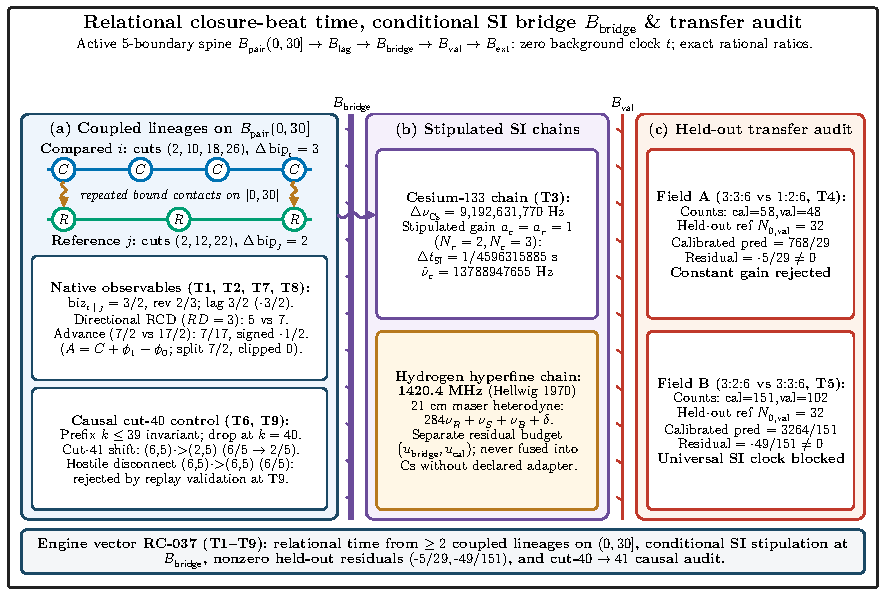
\includegraphics[width=0.92\linewidth,height=0.78\textheight,keepaspectratio]{figures/generated/temporal-si-bridge-feynman.pdf}
\caption{Coupled closure-beat lineages on half-open integer window $B_{\mathrm{pair}}(0,30]$, conditional Cesium/Hydrogen hyperfine SI bridge chains at $B_{\mathrm{bridge}}$, held-out cross-field transfer audit at $N_{0,\mathrm{val}}=32$, and cut-$40\to41$ causal control (\texttt{temporal\_si\_bridge\_dec\_ledger.csv}).}
\label{fig:manual-temporal-si-bridge-feynman}
\end{figure}

\begin{table}[H]
\centering
\caption{Engine-bound nine-stage relational closure-beat time, conditional SI bridge, held-out transfer, and cut-$40\to41$ causal audit ledger (\texttt{RC-037}, live from \texttt{temporal\_si\_bridge\_dec\_ledger.csv}).}
\label{tab:manual-temporal-dec-bridge}
{\scriptsize
\begin{tabular}{>{\raggedright\arraybackslash}p{0.133\linewidth}>{\raggedright\arraybackslash}p{0.133\linewidth}>{\raggedright\arraybackslash}p{0.206\linewidth}>{\raggedleft\arraybackslash}p{0.116\linewidth}>{\raggedleft\arraybackslash}p{0.120\linewidth}>{\raggedright\arraybackslash}p{0.150\linewidth}}
\toprule
Stage & Boundary $B$ & Lineage / anchor \& counts & Exact quantity & Reverse / resid & Gate status \\
\midrule
\texttt{T1\_\allowbreak{}pair\_\allowbreak{}closures} & B\_\allowbreak{}pair\allowbreak{}(0,\allowbreak{}30] & compared\allowbreak{}(2,\allowbreak{}10,\allowbreak{}18,\allowbreak{}26) vs ref\allowbreak{}(2,\allowbreak{}12,\allowbreak{}22)\par (3 vs 2) & 3/2 & 2/\allowbreak{}3 & AUTHENTICATED\_\allowbreak{}EXACT\_\allowbreak{}RCD \\
\texttt{T2\_\allowbreak{}unwrapped\_\allowbreak{}lag} & B\_\allowbreak{}pair\allowbreak{}(0,\allowbreak{}30] & bias\allowbreak{}(+1/\allowbreak{}4,\allowbreak{}-1/\allowbreak{}4)\par (1+1/\allowbreak{}2) & 3/2 & -3/\allowbreak{}2 & AUTHENTICATED\_\allowbreak{}EXACT\_\allowbreak{}LAG \\
\texttt{T3\_\allowbreak{}cs133\_\allowbreak{}bridge} & B\_\allowbreak{}bridge\allowbreak{}(a\_\allowbreak{}c=a\_\allowbreak{}r=1) & Cs\_\allowbreak{}9192631770Hz\par (N\_\allowbreak{}r=2,\allowbreak{}N\_\allowbreak{}c=3) & 1/4596315885 & 13788947655 & CONDITIONAL\_\allowbreak{}SI\_\allowbreak{}STIPULATED\_\allowbreak{}GAIN \\
\texttt{T4\_\allowbreak{}transfer\_\allowbreak{}field\_\allowbreak{}A} & B\_\allowbreak{}val\_\allowbreak{}A\allowbreak{}(32\_\allowbreak{}ref) & 3:3:6\_\allowbreak{}vs\_\allowbreak{}1:2:6\par (cal=58,\allowbreak{}val=48) & 768/29 & -5/\allowbreak{}29 & REJECTS\_\allowbreak{}CONSTANT\_\allowbreak{}TRANSFER \\
\texttt{T5\_\allowbreak{}transfer\_\allowbreak{}field\_\allowbreak{}B} & B\_\allowbreak{}val\_\allowbreak{}B\allowbreak{}(32\_\allowbreak{}ref) & 3:2:6\_\allowbreak{}vs\_\allowbreak{}3:3:6\par (cal=151,\allowbreak{}val=102) & 3264/151 & -49/\allowbreak{}151 & REJECTS\_\allowbreak{}CONSTANT\_\allowbreak{}TRANSFER \\
\texttt{T6\_\allowbreak{}cut40\_\allowbreak{}intervention} & B\_\allowbreak{}causal\allowbreak{}(cut40->\allowbreak{}41) & capacity\_\allowbreak{}drop\_\allowbreak{}control\par (\allowbreak{}(6,\allowbreak{}5)->\allowbreak{}\allowbreak{}(2,\allowbreak{}5)) & 6/5 & 2/\allowbreak{}5 & STRICTLY\_\allowbreak{}LATER\_\allowbreak{}CUT41\_\allowbreak{}RESPONSE \\
\texttt{T7\_\allowbreak{}directional\_\allowbreak{}rcd} & B\_\allowbreak{}rcd\allowbreak{}(RD=3) & c\_\allowbreak{}refs\allowbreak{}(1,\allowbreak{}1) vs r\_\allowbreak{}refs\allowbreak{}(2,\allowbreak{}2)\par (RCD\_\allowbreak{}c|r=5,\allowbreak{}RCD\_\allowbreak{}r|c=7) & 5 & 7 & AUTHENTICATED\_\allowbreak{}DIRECTIONAL\_\allowbreak{}RCD \\
\texttt{T8\_\allowbreak{}observed\_\allowbreak{}advance\_\allowbreak{}si} & B\_\allowbreak{}phase\allowbreak{}(A=C+phi1-phi0) & A\_\allowbreak{}c=7/\allowbreak{}2 vs A\_\allowbreak{}r=17/\allowbreak{}2\par (split=7/\allowbreak{}2;\allowbreak{}clip=0) & 7/17 & -1/\allowbreak{}2 & EXACT\_\allowbreak{}OBSERVED\_\allowbreak{}ADVANCE\_\allowbreak{}ADDITIVE \\
\texttt{T9\_\allowbreak{}causal\_\allowbreak{}disconnect\_\allowbreak{}control} & B\_\allowbreak{}causal\_\allowbreak{}hostile\allowbreak{}(prefix<=39) & disconnect\_\allowbreak{}feedback\_\allowbreak{}mutation\par (\allowbreak{}(6,\allowbreak{}5)->\allowbreak{}\allowbreak{}(6,\allowbreak{}5)) & 6/5 & REJECTED\_\allowbreak{}REPLAY\_\allowbreak{}VALIDATION & HOSTILE\_\allowbreak{}DISCONNECT\_\allowbreak{}REJECTED \\
\bottomrule
\end{tabular}
}
\end{table}
